\documentclass{article}

\RequirePackage[english]{babel}
\RequirePackage[utf8]{inputenc}
\RequirePackage[paper=a4paper, left=2cm, right=2cm, top=2cm, bottom=2cm]{geometry}
\RequirePackage[indent=0cm]{parskip}
\RequirePackage[colorlinks, linkcolor=blue, urlcolor=magenta, citecolor=green, bookmarks]{hyperref}
\RequirePackage{graphicx}
\RequirePackage{xcolor}
\RequirePackage{caption, subcaption}
\RequirePackage[separate-uncertainty = true]{siunitx}

\RequirePackage[backend=bibtex,
  citestyle=authoryear,
  style=alphabetic]{biblatex}
\addbibresource{bibliography.bib}


\RequirePackage{minted}
\newcommand{\ipy}[1]{\mintinline{python3}{#1}}

\title{
  {\normalsize Computing Methods for Experimental Physics and Data Analysis}\\
  Playing \emph{Connect-4} with Deep Neural Networks
}
\author{Luca Arnaboldi\footnote{Id. Number: 565650, Email: \href{mailto:l.arnaboldi@studenti.unipi.it}{l.arnaboldi@studenti.unipi.it}}}
\date{a.y. 2020-2021}

\begin{document}
  \maketitle
  \begin{abstract}
    The goal of this project is to train a DNN to play \emph{Connect 4}. Although the game has been completely solved many years ago, it still offers a really interesting environment where training and testing neural networks. First of all, I've implemented a game engine that allows playing games and tournaments between players based on many different classical strategies. After that, I've used the data collected from many games between the known agents, in order to train a convolutional neural network with supervised learning. In the end, I've explored reinforcement learning techniques to create a neural network that is able to play without relying on an external agent for training. 
  \end{abstract}
  
  \emph{Connect-4} is a game where two players challenge each other in making a connection of 4 checks on a \(6\times7\) board\footnote{More on \emph{Connect4} rules at \href{https://en.wikipedia.org/wiki/Connect_Four}{Wikipedia}.}. 
  Since it is a perfect information game and the number of states is relatively limited, the game can be completely solved through enchanted brute-force techniques. Nevertheless, it is interesting to address the problem using Deep Neural Networks, since standard algorithms allow to evaluate exactly the performance of the machine learning ones.
  
  \paragraph{Game Engine}
  The first thing to do is writing a game engine that allows playing the game, it asserts that each move is an allowed position and checks for the winner. I've chosen to code in \texttt{Python}. The 3 principal classes of the GameEngine are:
  \begin{itemize}
    \item \ipy{Board}: it handles the board and all the methods to modify and check it. It's not contained in \ipy{Game} class since some strategies need methods on the board, but not a complete game. 
    \item \ipy{Game}: it handles the alternation between players' moves by calling the proper methods on \ipy{Player} objects at the right time. 
    \item \ipy{Player}: it's an \emph{abstract class} that must be the base class of all players.
  \end{itemize}

  The second step is to code some players that play with a given strategy. There are four categories of players:
  \begin{itemize}
    \item \emph{Basic Players}: they implement players without a real strategy. We have:
      \begin{itemize}
        \item \ipy{RandomPlayer}: plays a random move between the allowed ones.
        \item \ipy{ConsolePlayer}: read the move from \texttt{stdin}.
        \item \ipy{FixedMovesPlayer}: plays a given sequence of moves. Used principally for unit testing.
      \end{itemize}
    \item \emph{Search Players}: these players are all based on the \emph{minimax algorithm} applied to the moves tree.
      Most of these players use the \emph{alpha-beta pruning} technique to speed up the exploration. In addition to the classic implementations, there is a version that uses a heuristic  move order, and another that adds up random noise to the moves score in order to make the strategy not deterministic.
      
      This category includes also the \ipy{PerfectPlayer}, which is nothing more than a wrapper for my engine of a \texttt{C++} implementation of a full search algorithm\cite{perfectsolvertutotial, perfectsolverimplementation}, that I've included in my repository as a submodule. 
    \item \emph{Combination Players}: players that combine the strategy of two or more other players.
    \item \emph{TensorFlow Players}: they play using board evaluation through a \textit{TensorFlow} model.
  \end{itemize}
  
  A screenshot of the game engine running a game it's reported in Figure~\ref{fig:screenshot}.
  \href{https://arn4.github.io/connect4/doc/}{Full documentation} of the game engine and players can be found on GitHub Pages branch of the project.
  
  \begin{figure}
    \centering
    
    \begin{subfigure}{0.45\textwidth}
      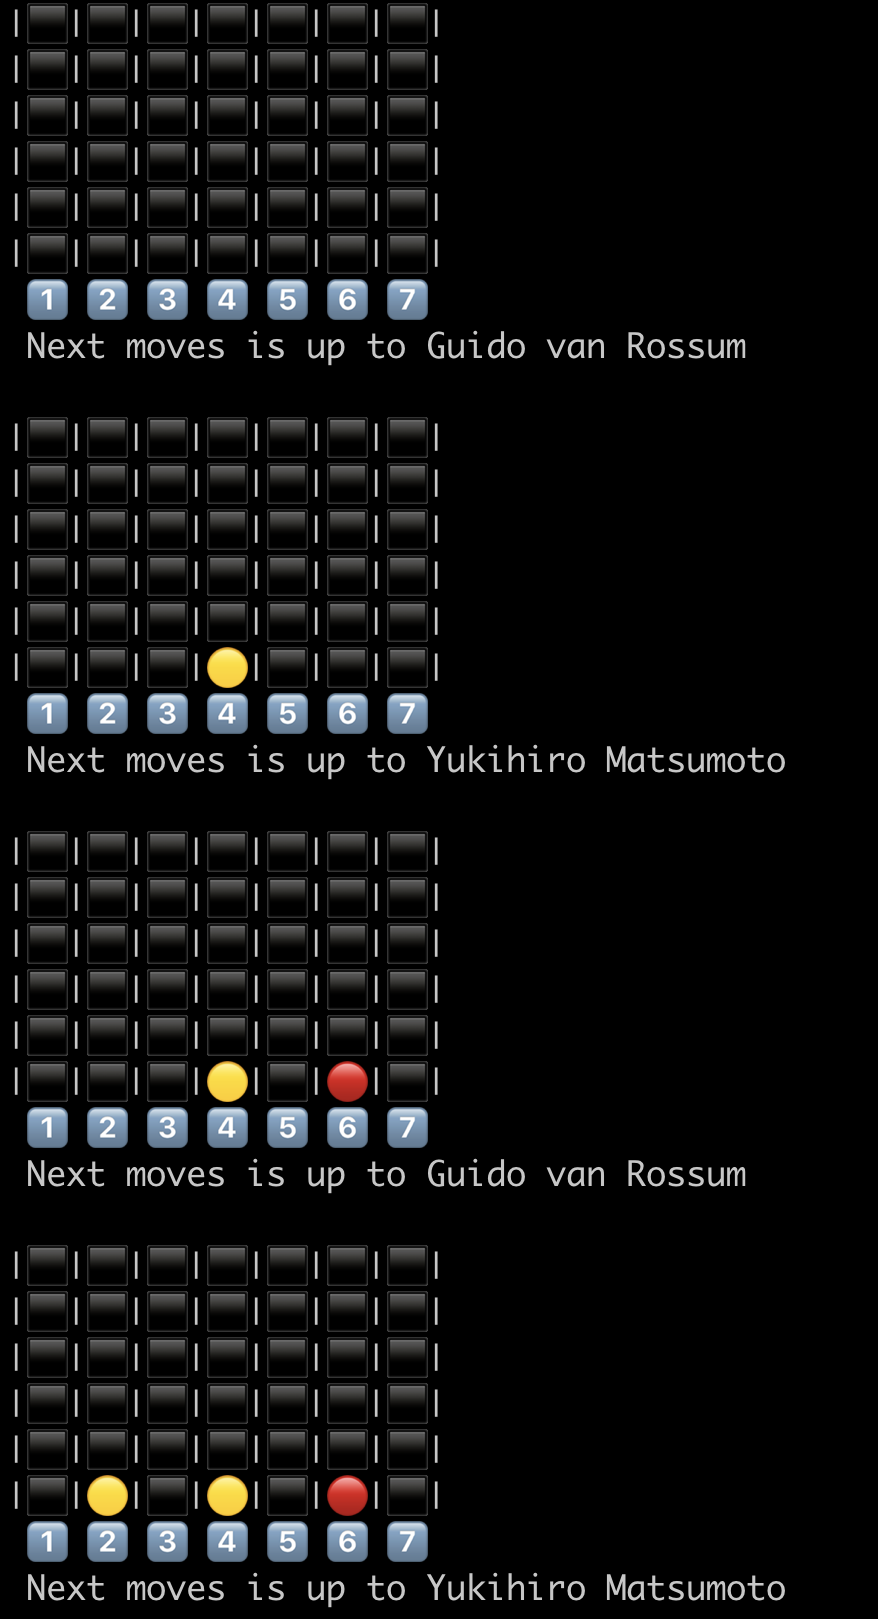
\includegraphics[width=\linewidth]{img/gamestart.png}
      \subcaption{}
    \end{subfigure}\hfil
    \begin{subfigure}{0.45\textwidth}
      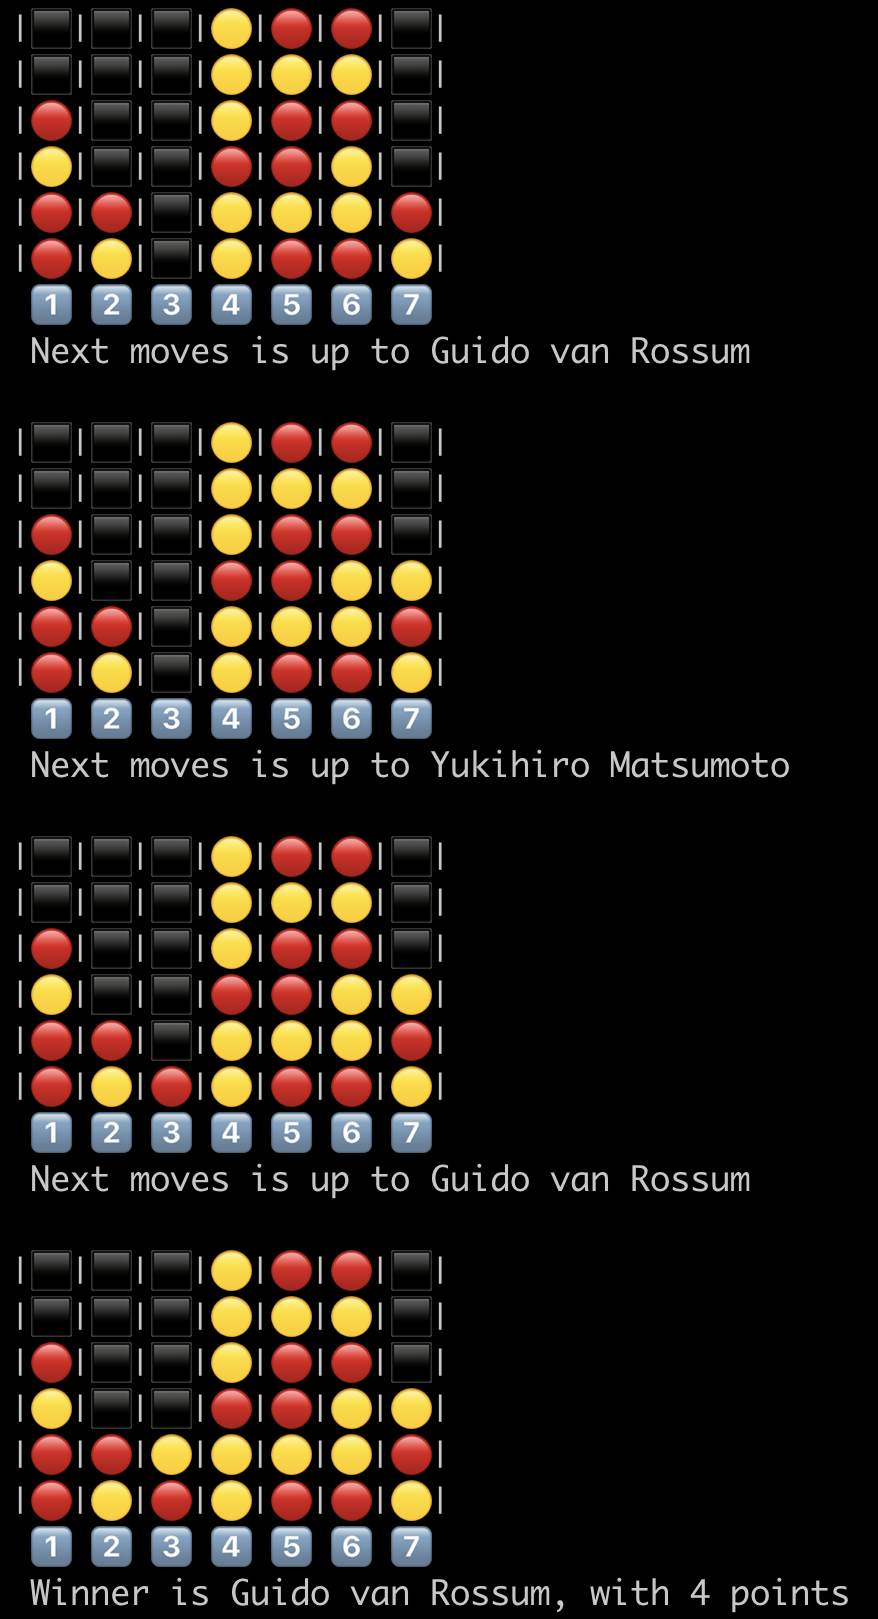
\includegraphics[width=\linewidth]{img/gameend.png}
      \subcaption{}
    \end{subfigure}
    \medskip
    
    \begin{subfigure}{0.9\textwidth}
      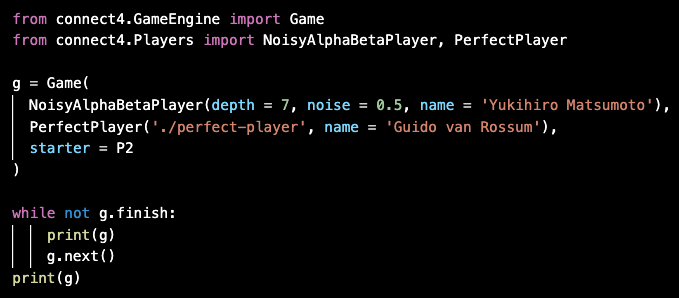
\includegraphics[width=\linewidth]{img/gamecode.png}
      \subcaption{}
    \end{subfigure}
    
    \caption{example of a game played with \ipy{connect4.GameEngine}. (a) beginning; (b) ending; (c) code that has generated the game.}
    \label{fig:screenshot}
  \end{figure}

  \paragraph{Supervised Learning}
  Once the setting is ready, we can start using DNN. The first approach I've tried is \emph{supervised learning}. I've coded a
  derived class of \ipy{GameEngine.Game} called \ipy{SupervisedGame} where a third player watches the game between other two, and stores the move it would do in every situation. The collected data is the dataset used for the training. I've collected the data from \(42000\) games between \ipy{RandomPlayer} and \ipy{NoisyAlphaBetaPlayer} with different noise and depth, all supervised by \ipy{CenteredAlphaBetaPlayer(6)}. Three corrections could be applied to the raw data:
  \begin{itemize}
    \item \emph{Symmetry}: the board is symmetric over vertical reflection. The symmetry can be applied to double the data in the dataset.
    \item \emph{Duplicates}: some board configurations can appear more than once; duplicates can be removed.
    \item \emph{Information Threshold}: the supervisor may not able to find the best moves in a configuration, resulting in a low information distribution that may be discarded.
  \end{itemize}
  Since the board has already a 2D structure I've decided to use a convolutional neural network, with a squared kernel size equal to 4. After the convolutional layer, there are 2 hidden layers with ReLU activation function, and finally the output layer has 7 (as the number of columns) neurons. Each output neuron value is the \texttt{logit} of the probability that the agent should move in that column. 
  I've trained the network for 300 epochs, using binary cross-entropy as loss function; the result of the training is shown in Figure~\ref{fig:supervisedresult}.
  \begin{figure}
    \centering 
    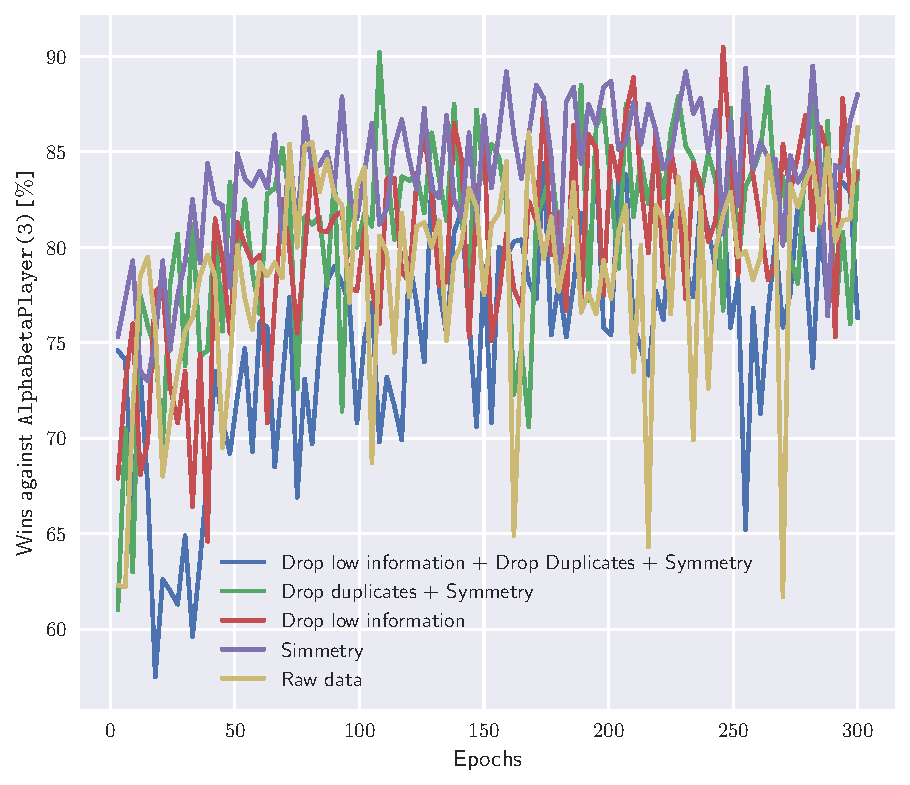
\includegraphics[width=0.7\textwidth]{img/supervised.pdf}
    
    \caption{result of supervised training.}
    \label{fig:supervisedresult}
  \end{figure}
  Although the figure is a little bit messy, it can be still seen that a better performance is achieved when only the symmetry is applied to the dataset; this is reasonable because it's the situation where the number of testcases is larger. Dropping the duplicates or the low information boards changes the data distribution to a different one than the one encountered while playing real games. 
  
  The last thing that can be done is to test the best-trained model against the supervisor used to generate the dataset. Testing over 1000 matches, the supervised agent won only \(15.4\si{\percent}\) of them. As expected the supervisor performs better than the trained network, which is still far from reaching its level.
  
  \paragraph{Reinforcement learning}
  Supervised Learning is a bit like cheating if the goal is to create a stand-alone player who can play using a neural network. This is because we need a player which is able to play reasonably well to generate the dataset. To train a neural network without any external agent we have to use \emph{reinforcement learning}. The approach I've decided to take is a revisited version of \emph{deep Q-learning}: I train a DNN that is able to assign a score to each board configuration, and the agent makes the move that gives the highest score. In each episode, the agent plays against itself and the configuration scores are calculated based on the game result when the match is finished. As in supervised learning, the horizontal symmetry can be used to double the number of testcases. The \emph{epsilon-greedy strategy} is used to deal with the trade-off between learning and exploration. The loss function used is mean squared error. A few things can still be configured:
  \begin{itemize}
    \item \emph{Epsilon decay}: the decay of \(\varepsilon\) over episodes can be linear or exponential. The difference can be seen in Figure~\ref{fig:decays}. 
    \item \emph{Flattened Neural Network}: it could be that a not convolutional neural network learns better.
    \item \emph{Multi-Traning}: it may happen that an agent adapt to play only against himself and does not learn a good general strategy. This could be avoided by training 2 or more agents together.
  \end{itemize}
  \begin{figure}
    \centering
    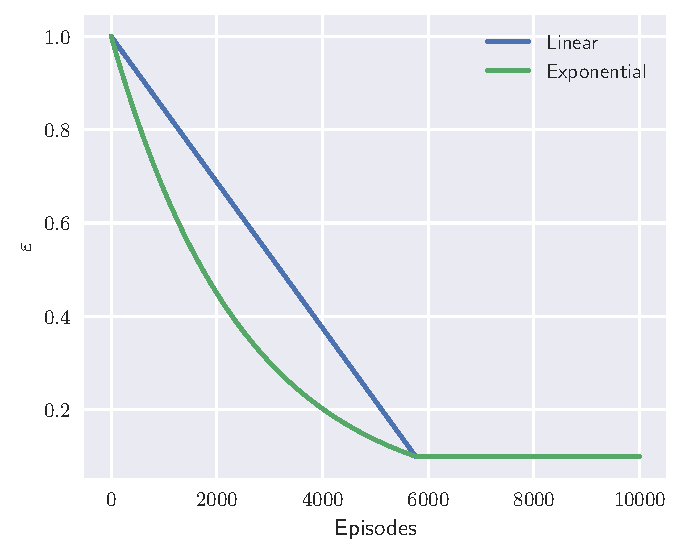
\includegraphics[width=0.7\textwidth]{img/decay.pdf}
    
    \caption{two possible \(\varepsilon\)-decays over 10000 episodes. A minimum value of \(\varepsilon\) has been set since some tests showed that too low \(\varepsilon\) are useless to learning.}
    \label{fig:decays}
  \end{figure}

  I've tested all these hypotheses and the results are shown in Figure~\ref{fig:reinforcement10k}. It's clear that the flattened neural network is worse than all the others, so the initial choice of using a convolutional one is correct. There is no appreciable difference between linear and exponential decay, but since the former makes the learning faster, the linear one is preferable.
  \emph{Multi-training} does not significantly boost learning, but it outputs three independent models that can be combined with \ipy{PoolPlayer}\footnote{\ipy{PoolPlayer} combines a group of indipendent players ysing majority voting.}. Moreover, training more than one agent does not affect the performance too much since most of the jobs can be parallelized.
 
  I've decided to go with a 50000 episodes multi-training of 3 agents, with linear decay. The result is plotted in Figure~\ref{fig:reinforcement50k}. As already seen in the 10000 training, the performance peaks after a relatively small part of the learning and starts dropping after that. This could be a manifestation of \emph{catastrophic forgetting}\cite{kirkpatrick2017overcoming}: after early stages of learning the agents start to explore different game phases and forget how to deal with early the stages of the match, resulting in a performance decrease. Dealing with these kinds of problems is beyond the scope of this project; the simplest thing we can do is combine the 3 agents by picking their best performance. Using a \ipy{PoolPlayer} we get a \(57.0\si{\percent}\) against \ipy{AlphaBetaPlayer(3)}.
  
  \paragraph{Conclusions} None of the two training methods led to a superhuman performance in the game.
  
  Supervised learning can be improved by using a stronger supervisor, but it would cost much more time for generating the dataset. As already pointed out, invest computational time in supervised learning is not that useful since the supervisor would always play better than the trained network.
  
  Reinforcement learning has much room for improvement. Besides loss function and optimizer that can be changed,
  the learning strategy can probably include a phase where the DNN faces against some classical players. This may prevent catastrophic forgetting and let the agent explore some phases of the game that would never be reached otherwise.
  To top it off, using more computational resources could only benefit learning.
  
  Watching the RL agent playing, it's clear that it lacks the ability of predicting the moves of the opponent. 
  Probably a really good and fast player would be obtained by combining the alpha-beta pruning algorithm with the evaluation of the board by the NN.
  In my opinion the combination of exploring and ability to estimate the goodness the position would be the perfect mix to reach human performance, or even better.
  
  

  \begin{figure}
    \centering
    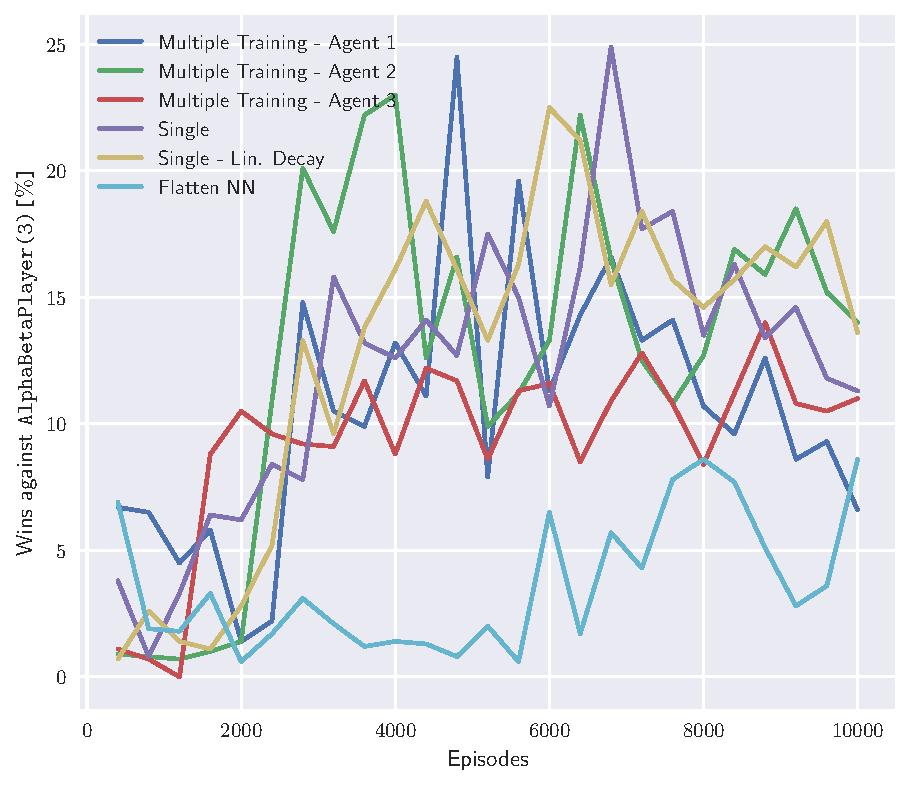
\includegraphics[width=0.7\textwidth]{img/reinforcement-10k-comparsion.pdf}
    
    \caption{test different training strategy of Reinforcement Learning with 10000 episodes.}
    \label{fig:reinforcement10k}
  \end{figure}

  \begin{figure}
    \centering
    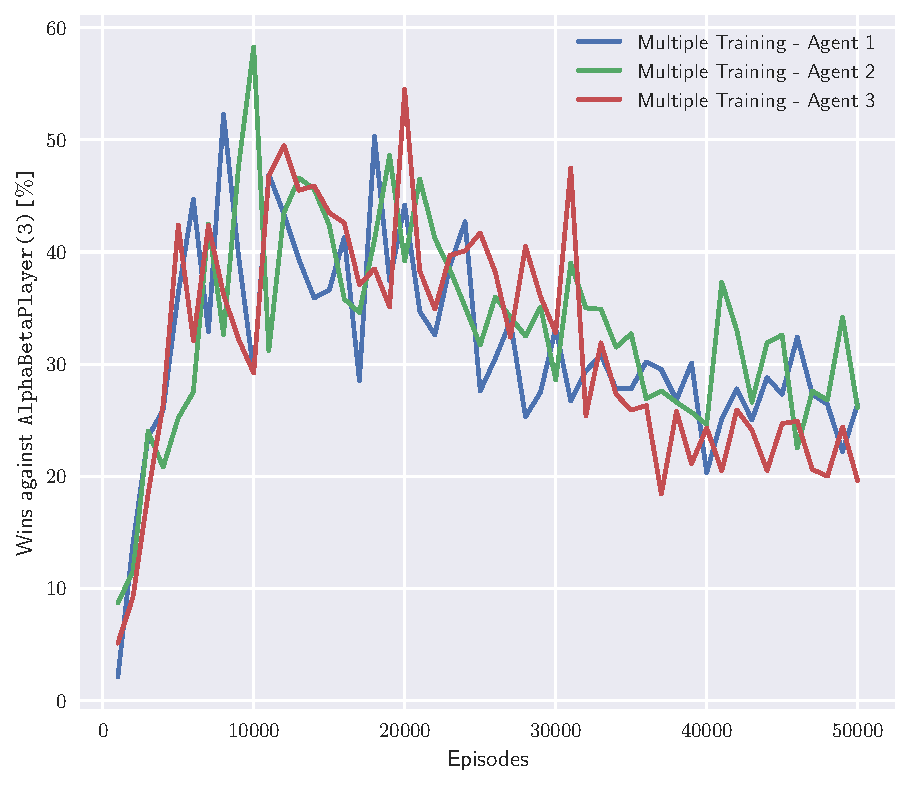
\includegraphics[width=0.7\textwidth]{img/reinforcement-50k.pdf}
    
    \caption{result of supervised training.}
    \label{fig:reinforcement50k}
  \end{figure}



  \printbibliography
\end{document}
